%Elliptische Kurven
\chapter{Elliptische Kurven}


Als Basis für asymmetrische Kryptosysteme können elliptische Kurven dazu genutzt werden, die verschlüsselungstechnische Effektivität mathematischer Probleme, wie das des diskreten Logarithmus, zu erhöhen. Bei der Kryptographie unter Verwendung elliptischer Kurven, kann mit deutlich kürzerer Schlüssellänge ein gleichwertiges Ergebnis erzielt werden. Dieser Effekt wird durch die spezielle Arithmetik auf elliptischen Kurven erzielt, deren mathematische Grundlage, konkrete Eingenschaften und Funktionsweise im folgenden Kapitel erörtert werden soll.\\

Elliptische Kurven können über beliebigen Körpern definiert werden. Für die Kryptographie interessant sind elliptische Kurven über Primkörpern.\\

%\section{Definition: Elliptische Kurven}
% Sei \textit{p} eine \textit{Primzahl} $p>3$. Seien $a,b \in GF(p)$. Betrachte die Gleichung
%\begin{equation}
%    y^2 z = x^3 + axz^2 + bz^3.\label{eq:g1}
%\end{equation} Die \textit{Diskriminante}  dieser Gleichung ist
%\begin{equation}
%    \delta = -16(4a^3 + 27b^2).\label{eq:g2}
%\end{equation}
%Wir nehmen an, dass die Diskriminante $\delta$ nicht Null ist. Ist $(x,y,z) \in GF(p)^3$ eine Lösung dieser
%Gleichung, so ist für alle $c \in GF(p)$ auch $c(x,y,z)$ eine solche Lösung. Zwei Lösungen $(x,y,z)$ und $(x',y',z')$
%heißen \textit{äquivalent}, wenn es ein von Null verchiedenes $c \in GF(p)$ gibt mit $(x,y,z) = c(x',y',z')$. Dies
%definiert eine Äquivalenzrelation auf der Menge aller Lösungen der~\eqref{eq:g1}.




Um das weitere Verständnis zu verbessern, wollen wir erst eine uns schon bekannte Kurve ansehen. In Abbildung \ref{fig:Einheitskreis} ist das Polynom $x^2 + y^2 = r^2$ über $\mathbb{R}$ dargestellt. Wie zu sehen ist, handelt es sich hierbei um die Kreisgleichung. Der zu sehende Kreis ist nichts anderes als die Menge aller Punkte, welche die Kreisgleichung erfüllen.
Ein Beispiel für eine solchen ist der Punkt $(r,0)$. Wenn $x$ den Wert $r$ hat, muss $y$ folglich den Wert $0$ haben. Ein Gegenbeispiel ist der Punkt $(r,r/2)$. Dieser erfüllt die Kreisgleichung nicht.
\begin{figure}[!h]
    \centering
    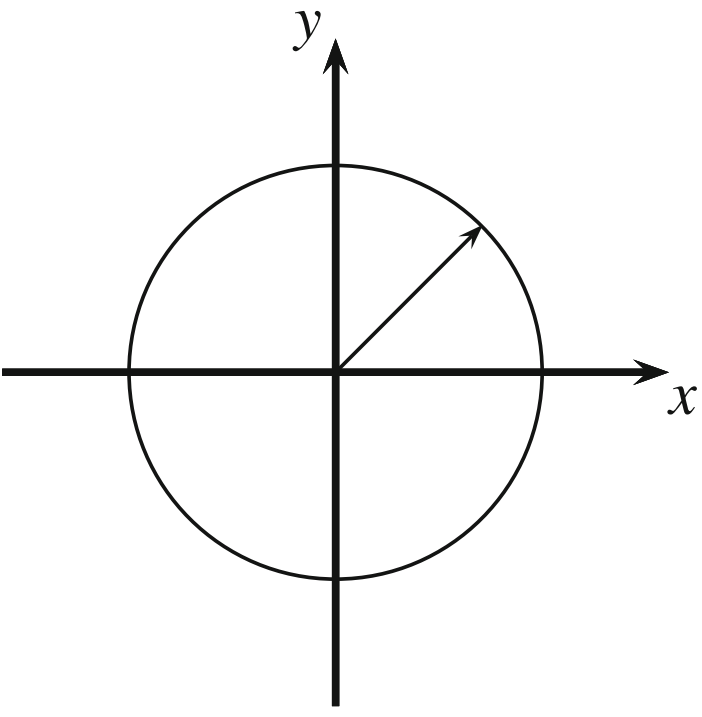
\includegraphics[width=0.3\textwidth]{grafiken/Kreis.PNG}
    \caption{Einheitskreis}
    \label{fig:Einheitskreis}
\end{figure}
Die Kreisgleichung kann verallgemeinert werden, indem den Termen $x^2$ und $y^2$ Koeffizienten voran gesetzt werden. Eine solche Gleichung, $ax^2 + by^2 = c$ erzeugt über $\mathbb{R}$ eine Ellipse, wie in Abbildung \ref{fig:Ellipse} zu sehen.
\begin{figure}[H]
    \centering
    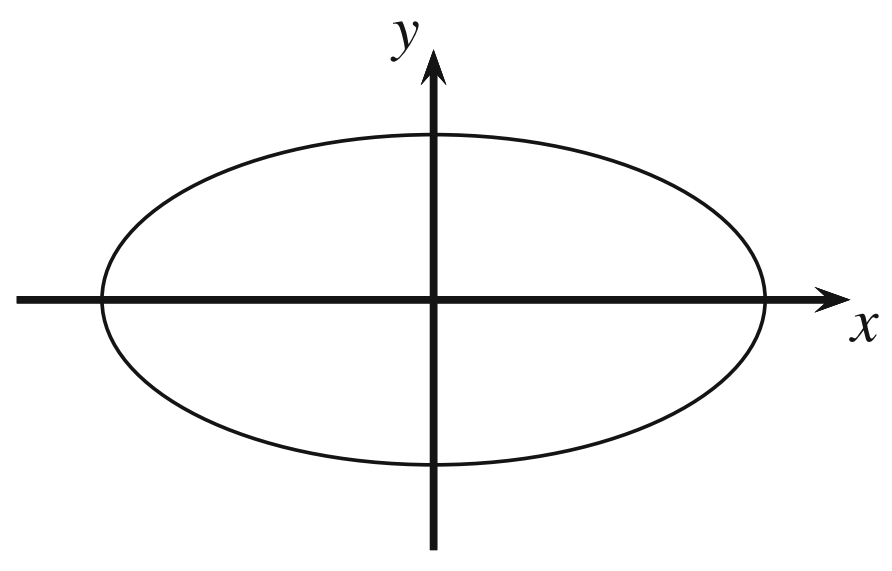
\includegraphics[width=0.3\textwidth]{grafiken/Ellipse.PNG}
    \caption{Ellipse}
    \label{fig:Ellipse}
\end{figure}
Eine elliptische Kurve ist nun eine spezielle Polynomgleichung, der Form $y^2 = x^3 + ax + b$, unter der Bedingung $4a^3 + 27b^3 \neq 0$. Eine solche Gleichung über $\mathbb{R}$ ist in Abbildung \ref{fig:Elliptische_Kurve} dargestellt.
\begin{figure}[!h]
    \centering
    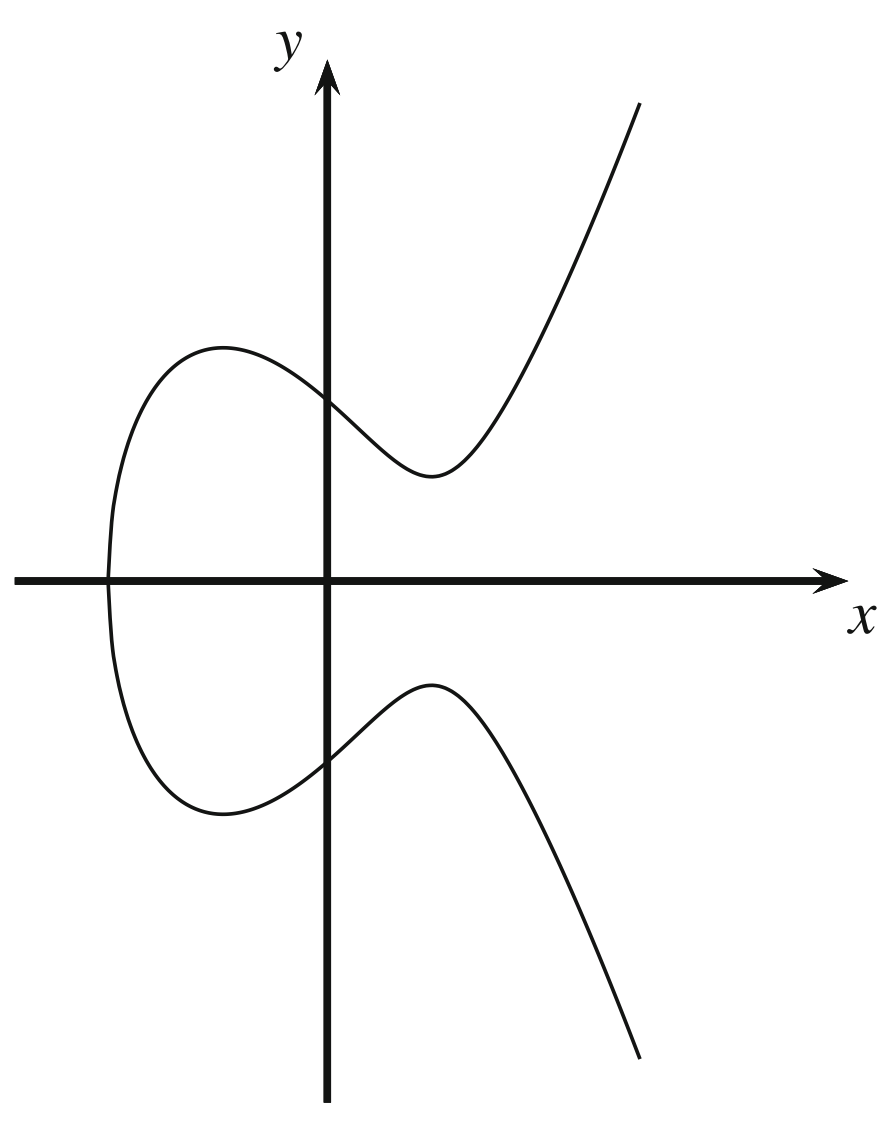
\includegraphics[width=0.3\textwidth]{grafiken/Elliptische_Kurve.PNG}
    \caption{Elliptische Kurve}
    \label{fig:Elliptische_Kurve}
\end{figure}
Damit elliptische Kurven sinnvoll in der Kryptologie eingesetzt werden können, muss die Polynomgleichung über einem Primkörper betrachtet werden. Das heißt einfach gesprochen, alle Berechnungen werden modulo $p$ durchgeführt.
\paragraph{Definition: Elliptische Kurven über Primkörpern}
Die \textit{elliptische Kurve} über $\mathbb{F_p}$, ist die Menge aller Punkte $(x,y)$ mit $x,y \in \mathbb{F_p}$, welche die folgende Gleichung erfüllen: 
\begin{center}
$y^2 \equiv x^3 + ax + b$ mod $p$, wobei $a,b \in \mathbb{F}_p$
\end{center} 
und die Bedingung
\begin{equation}
3 + 27b^3 \neq 0
\label{eq:constraint}
\end{equation} gelten müssen. Zu der elliptischen Kurve gehört des Weiteren auch der imaginäre \textit{Punkt im Unendlichen} $\mathcal{O}$.\\

Durch die Bedingung \ref{eq:constraint} werden sog. Singularitäten ausgeschlossen. Andernfalls gäbe es Punkte, deren Tangente nicht eindeutig definiert ist, was für das Rechnen auf elliptischen Kurven jedoch erforderlich ist.\cite[273-276]{Paar.2016}

\section{Arithmetik} \label{sec:Arithmetik}
Nachdem elliptische Kurven nun definiert wurden, stellt sich die Frage, wie diese in der Kryptographie eingesetzt werden können. Wenn wir uns an das in Kapitel \ref{sec:Das_diskrete_Logarithmusproblem} zurückerinnern, wird für die Konstruktion eines \textbf{DLP}s eine zyklische Gruppe benötigt. Eine eben solche findet sich in der Punktmenge der elliptischen Kurve wieder. Offen bleibt wie die Gruppenoperation definiert ist. Diese muss die in Kapitel \ref{sec:gruppe} geforderten Gruppengesetze erfüllen.\\

Als Symbol für die Gruppenoperation wird das Additionszeichen $+$ verwendet. Durch die Gruppenoperation muss aus zwei Punkten $P = (x_1, y_2)$ und $Q= (x_2, y_2)$ der Kurve ein dritter Punkt $R$ auf der Kurve berechnet werden. 
$$P + Q = R$$ $$(x_1, y_1) +  (x_2, y_2) = (x_3, y_3)$$
Am verständlichsten lässt sich diese Operation grafisch zeigen. Elliptische Kurven über endlichen Körpern können grafisch nicht sinnvoll dargestellt werden. Ihre Form und Arithmetik lassen sich jedoch gut veranschaulichen wenn man sie auf $\mathbb{R}$ abbildet. Im Folgenden betrachten wir eine Elliptische Kurve, dargestellt in einem kartesischen Koordinatensystem, um die Gruppeneigenschaften bezüglich der Punktaddition zu zeigen. Hierbei sind nun zwei Fälle zu unterscheiden.\\

\paragraph{Punktaddition $P + Q$:}
Falls $P \neq Q$ erfolgt die geometrische Konstruktion, indem zunächst eine Grade durch die beiden Punkte gelegt wird. Aufgrund der Kurveneigenschaften hat diese im Normalfall einen dritten Schnittpunkt mit der Kurve. Dieser wird an der $x$-Achse gespiegelt um den gesuchten Punkt $R$ zu erhalten. Abbildung \ref{fig:Punktaddition} zeigt die beschriebene Konstruktion.

\begin{figure}[H]
    \centering
    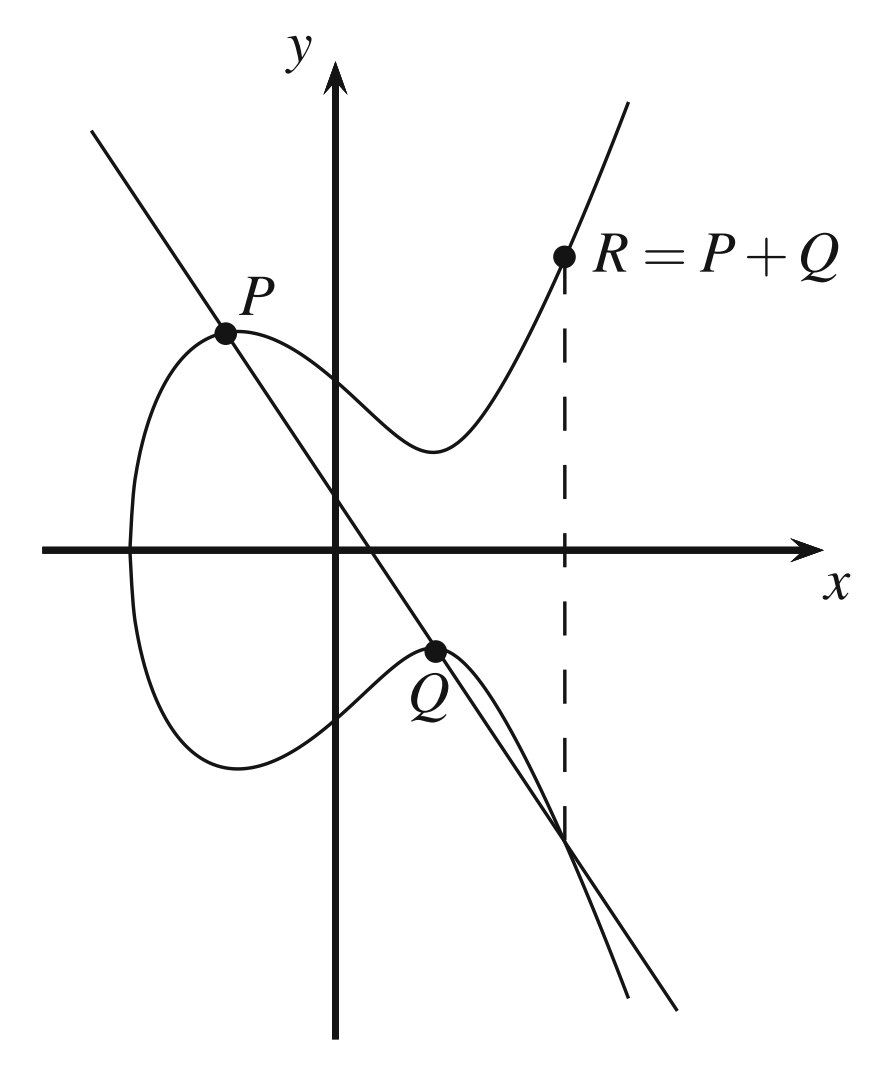
\includegraphics[width=0.3\textwidth]{grafiken/Punktaddition.PNG}
    \caption{Punktaddition}
    \label{fig:Punktaddition}
\end{figure}

\paragraph{Punktverdopplung $P + P$:}
Falls P und Q identisch sind erfolgt die geometrische Konstruktion, indem eine Tangente an den Punkt $P$ angelegt wird. Diese liefert wieder einen weiteren Schnittpunkt mit der Kurve, welcher an der $x$-Achse gespiegelt wird um den Punkt $R$ zu erhalten. Anstatt $R = P + Q$ schreibt man in diesem Fall $R = P + P = 2P$   Abbildung \ref{fig:Punktverdopplung} zeigt die beschriebene Konstruktion. 

\begin{figure}[H]
    \centering
    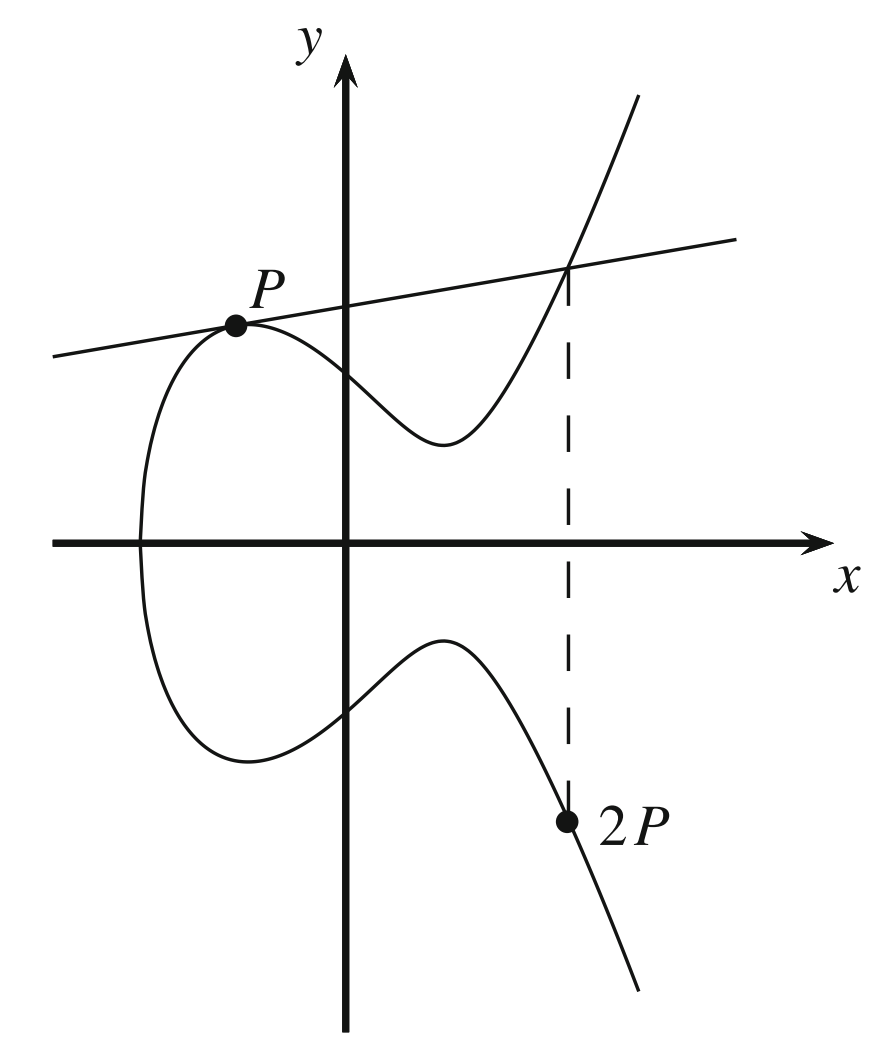
\includegraphics[width=0.3\textwidth]{grafiken/Punktverdopplung.PNG}
    \caption{Punktverdopplung}
    \label{fig:Punktverdopplung}
\end{figure}

\paragraph{Sonderfall $P + (-P)$:}
In beiden genannten Fällen, Punktaddition und Punktverdopplung, kann es passieren, dass es keinen weiteren Schnittpunkt mit der Kurve gibt. Dieser Fall tritt für die Punktaddition ein, wenn die $x$-Koordinaten der Punkte identisch sind. Für die Punktverdopplung tritt der Fall ein, wenn die $y$-Koordinate Null ist. In beiden Situationen ergibt sich für die Gerade, welche den genannten Schnittpunkt liefern soll, eine Parallele zur $y$-Achse. Diese schneidet die elliptische Kurve nicht mehr. Abbildung \ref{fig:UnendlichFernerPunkt} zeigt den Sonderfall für die Punktaddition. Als Ergebnis in einem solchem Fall wird der \textit{unendlich ferne Punkt} $\mathcal{O}$ definiert. Dieser hat noch weitere Eigenschaften im Bezug auf die Gruppeneigenschaften, welche im Kapitel \ref{sec:Gruppeneigenschaften} genauer erläutert werden.

\begin{figure}[H]
    \centering
    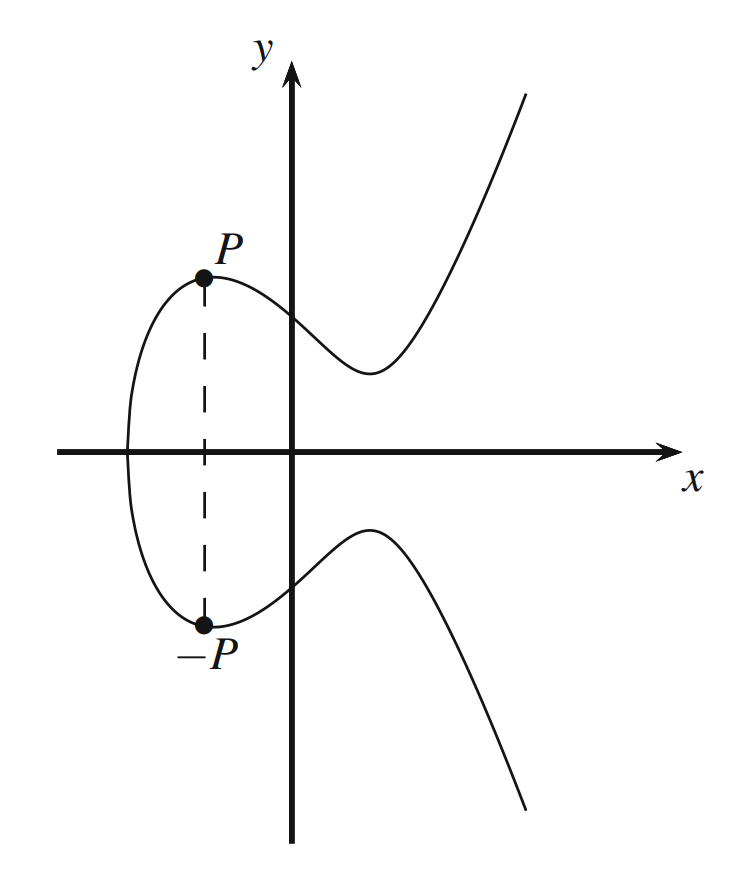
\includegraphics[width=0.3\textwidth]{grafiken/UnendlichFernerPunkt.PNG}
    \caption{Unendlich ferner Punkt}
    \label{fig:UnendlichFernerPunkt}
\end{figure}

Nach dieser grafischen Veranschaulichung sollte es leichter fallen die folgenden Formeln für die Punktaddition bzw. Punktverdopplung nachvollziehen zu können. Die Gruppenoperation existiert in jedem Körper, weshalb die Berechnung von $R$, wie grade gezeigt über den reellen Zahlen $\mathbb{R}$, als auch über einem Primkörper $\mathbb{F}_p$ durchgeführt werden kann.\cite[276-280]{Paar.2016}\\

Die Formeln für die Punktaddition und - verdopplung auf elliptischen Kurven können anhand der grade gezeigten Veranschaulichung hergeleitet werden.\\ 

\paragraph{Herleitung: Formeln für Punktaddition bzw. Punktverdopplung}
Gegeben ist die Gleichung der elliptischen Kurve $y^2 = x^3 +ax + b$ und die Punkte $P = (x_1, y_1)$ und $Q = (x_2, y_2)$. Zunächst ist die Geradengleichung der Sekante durch $P$ und $Q$ zu ermitteln. Eine Grade im Allgemeinen hat die Form $$g: y = sx + m.$$ Der Parameter $s$ ist dabei die Steigung der Geraden und $m$ ist der Schnittpunkt mit der $y$-Achse. Die Steigung $s$ lässt sich (im Fall der Punktaddition) wie gewohnt durch Anlegen des Steigungsdreiecks berechnen, also mit der Formel $$s = \frac{y_2 - y_1}{x_2  - x_1}.$$ Im Falle einer Punktverdopplung muss $s$ über die Tangente der Elliptischen Kurve im entsprechenden Punkt ermittelt werden. Dazu leiten leiten wir die Kurvengleichung der elliptischen Kurve nach $x$ ab. Es ergibt sich $$\frac{\delta y}{\delta x} = \frac{3x^2 + a}{2 \sqrt{x^3 + ax + b}}.$$ Bei genauerer Betrachtung fällt auf, dass der Nenner genau $2y$ entspricht, weshalb auch $$\frac{\delta y}{\delta x} = \frac{3x^2 + a}{2y}$$ geschrieben werden kann. Da die erste Ableitung die Steigung der elliptischen Kurve in jedem Punkt beschreibt, haben wir somit eine Formel mit welcher wird durch einsetzen eines Punktes $P = (x_1, y_1)$, die jeweilige Tangentensteigung ermitteln können. Es gilt also $$s = \frac{3x_1^2 + a}{2y_1}\text{.}$$

Zur Bestimmung des Schnittpunkts mit der $y$-Achse kann nun einer der beiden Punkte $P$ oder $Q$ in die Geradengleichung $y = s \cdot x + m$ eingesetzt werden. Durch Einsetzen des Punkts $P = (x_1, y_1)$  erhalten wir die folgende Gleichung $$y_1 = s \cdot x_1 + m\text{,}$$ welche nach $m$ aufgelöst folgendermaßen aussieht: $$m = y_1 - s \cdot x_1$$
Durch Einsetzten aller Parameter in die obige Geradengleichung ergibt sich $$y = \frac{y_2 - y_1}{x_2  - x_1} \cdot x + y_1 - \frac{y_2 - y_1}{x_2  - x_1} \cdot x_1$$ für die gesuchte Gerade $g$ durch die Punkte $P$ und $Q$. Um den dritten Schnittpunkt dieser Geraden $g$ mit der elliptischen Kurve $E$ zu ermitteln, sind beide Kurven gleichzusetzen. Da es für das weitere Vorgehen keine Rolle spielt und es der Übersichtlichkeit dient, werden im Folgenden wieder die Parameter $s$ und $m$ statt eben gezeigten Konkretisierungen verwendet. Es ergibt sich die Gleichung $$(sx+m)^2 = x^3 + ax + b\text{.}$$ Nach ausmultiplizieren der Gleichung erhalten wir $$0 =  x^3 - s^2x^2 + (a-2sm)\cdot x - m^2+b \text{.}$$

Im Normalfall ist das allgemeine Lösen eines solchen kubischen Polynoms nicht trivial. Wir haben hier jedoch den Vorteil, dass zwei der drei Schnittpunkte von $g$ mit $E$ schon bekannt sind. Fassen wir das Polynom als Funktion $$f(x) = x^3 - s^2x^2 + (a-2sm)\cdot x - m^2+b$$ auf, so sind wir Im Grunde auf der Suche nach den Nullstellen dieser kubischen Funktion. Da die Punkte $P$ und $Q$ auf der Geraden $g$ sowie auf der elliptischen Kurve $E$ liegen, lösen sie die obige
Gleichung, sind also Nullstellen der Funktion $f(x)$. Daraus folgt, dass die Funktion $f(x)$ restlos durch $(x-x_1)$ und $(x-x_2)$ geteilt werden kann um den Funktionsgrad zu verringern.
$$f(x) \div (x-x_1) \cdot (x-x_2) = l(x) \text{  Rest }0$$
Aufgrund dessen, dass $f(x)$ den Grad 3 hat, muss $l(x)$ den Grad 1 haben und durch $l(x) = ux + v$ beschrieben werden können. Da $$l(x) + (x-x_1) \cdot (x-x_2) = g(x)\text{,}$$ muss auch gelten $$u \cdot x \cdot x \cdot x  = x^3\text{,}$$ weshalb $u = 1$ gelten muss. Daraus ergibt sich $$l(x) = x + v \text{.}$$ Somit ist $x_3 = -v$ eine weitere Nullstelle von $f(x)$. Es folgt also $$g(x) = (x-x_1) \cdot (x-x_2) \cdot (x-x_3) \text{,}$$ woraus durch ausmultiplizieren $$f(x) = x^3 - (x_1 + x_2 + x_3) \cdot x^2 + (x_1 x_2 + x_1 x_3 + x_2 x_3) * x - x_1 x_2 x_3$$ entsteht. Vergleicht man nun diese Darstellung mit der obigen also $$f(x) = x^3 - s^2x^2 + (a-2sm)\cdot x - m^2+b\text{,}$$ so folgt durch Koeffizientenvergleich $$s^2 = x_1 + x_2 +x_3$$ also $$x_3 = x^2 -x_1 - x_2.$$

Um die Formel für $y_3$ zu ermitteln kann nun der Punkt $R$ in die Formel für $s$ eingesetzt werden. Dies ist möglich, da der Punkt $R$ auf der gleichen Geraden wie $P$ und $Q$ liegt, weshalb auch die Steigung $s$ identisch ist.
Es gilt also $$s = \frac{y_2 - y_1}{x_2  - x_1} = \frac{y_3 - y_1}{x_3  - x_1}.$$ 
Aufgelöst nach $y_3$ ergibt sich $$y_3 = s \cdot (x_3 - x_1) + y_1 \text{.}$$
Da der Schnittpunkt an der $x$-Achse gespiegelt wird um $R$ zu erhalten müssen die Vorzeichen in der Formel für $y$ noch gedreht werden. Final ergeben sich für den Punkt $R = (x_3, y_3)$ also die Formeln:
$$x_3 = s^2 + x_1 - x_2$$
$$y_3 = s \cdot (x_1 - x_3) - y_1$$


\paragraph{Formel: Punktaddition und -verdopplung auf elliptischen Kurven\cite[278]{Paar.2016}:}
$$x_3 = s^2 - x_1 - x_2$$
$$y_3 = s(x_1 - x_3) - y_1$$,
wobei

$$s = \begin{cases}
	\frac{y_2 - y_1}{x_2 -x_1} & \text{, falls } P \neq Q \text{ (Punktaddition)}\\
	\frac{3x_1^2 + a}{2y_1} & \text{, falls } P = Q \text{ (Punktverdopplung)}
	\end{cases}
$$

\section{Gruppeneigenschaften} \label{sec:Gruppeneigenschaften}
Zur Erfüllung der Gruppeneigenschaften wird außerdem ein neutrales Element $\mathcal{O}$ benötigt. Alle Punkte $P$ der elliptischen Kurve müssen die Eigenschaft $P + \mathcal{O} = P$ erfüllen. Da kein Punkt der elliptischen Kurve diese Eigenschaft erfüllen kann, wird der imaginäre \textit{unendlich ferne Punkt} als neutrales Element $\mathcal{O}$ definiert. Dieser Punkt liefert außerdem den \textit{Schnittpunkt} im oben genannten Sonderfall, also falls ein Punkt $P$ und der bezüglich der $x$-Achse gegenüberliegende Punkt $-P$ addiert werden. Die hier verwendete Terminologie $-P$ ist schon ein wenig voraus gegriffen, denn die Existenz eines neutralen Elements $\mathcal{O}$ ermöglicht nämlich die Definition eines Inversen $-P$ für jeden Punkt $P$ auf der Kurve. Laut der allgemeine Gruppengesetze gilt $$P + (-P) = \mathcal{O}.$$
Folgend aus der im vorigen Kapitel \ref{sec:Arithmetik} erläuterten Arithmetik auf elliptischen Kurven ist das Inverse eines Punktes $P = (x_p, y_p)$ der Punkt $-P = (y_p, -y_p)$, also der bezogen auf die $x$-Achse gegenüberliegende Punkt. In einem Primkörper berechnet sich die negative $y$-Koordinate durch $-y_p = p - y_p$.\cite[279]{Paar.2016}

 
\section{Punktbestimmung}
Die Arithmetik für Elliptische Kurven wurde bereits besprochen. Nun wird erarbeitet, wie man die Punkte einer elliptischen Kurve bestimmt. Doch was ist ein Punkt einer elliptischen Kurve? Im Foglenden wird erklärt, was ein Punkt auf einer elliptischen Kurve ist und wie diese berehcnet werden können. Die Erklärungen werden anschließend anhand einiger Beispiele näher erläutert. Anschließend wird Python-Code präsentiert, welcher die Punktbestimmung für eine elliptische Kurve mit p > 3 durchführt und die Punkte anschließend in der Konsole ausgibt.

\subsection{Rechnerische Grundlagen}
Viele Mathematiker suchten eine Formel, mit denen sich die Anzahl der Punkte einer elliptischen Kurve schätzen lässt, ohne dass man diese vorher aus- oder berechnen muss. Joseph H. Silverman beweist in seinem Buch einen mathematischen Satz aus der Zahlentheorie, welcher eine allgemeine Aussage über die Anzahl der rationalen Punkte auf einer elliptischen Kurve trifft \cite[138]{JosephH.Silverman.2009}. Dieser Satz kann also herangezogen werden, um eine ungefähre Abschätzung über die Anzahl der Punkte auf einer elliptischen Kurve über einem Primkörper p zu treffen. Bei dem mathematischen Satz handelt es sich um die Hasse–Weil–Schranke. Diese wird im allgemeinen dafür benutzt, um die Anzahl der Lösungen der Gleichung und der Bedingungen aber auch für die Einschränkung des Lösungsraums. Die Hasse-Weil-Schranke wird angelehnt an \cite[vgl.][S. 181]{reinholdhuebl} wie folgt beschrieben. Sei $k = \mathbb{F}_p$ ein endlicher Körper und $\overline{E}$ eine elliptische Kurve über k, dann gilt
\begin{center}
$p + 1 - 2 \cdot \sqrt{p} \leq | \overline{E} | \leq p + 1 + 2 \cdot \sqrt{p}$
\end{center} 

Was ist jedoch die Hauptaussage der Hasse-Weil-Schranke? Sie besagt, dass sich bei großen p die Anzahl der Elemente der elliptischen Kurve in der Größenoprdnung von p bewegen. Diese Schranke bildet hierbei eine obere und untere Grenze. Die Anzahl der Punkte bewegt sich also innerhalb dieser Schranke. Dies ist für elliptische Kurven mit kleinem p uninteressant, jedoch wird diese Schranke für elliptische Kurven mit großem gewählten p, was in der Kryptographie gängig ist, relevant.\\


Doch wie lassen sich die Punkte konkret berechnen? Um diese Frage zu beantworten, müssen wir noch einmal die Grundlagen für elliptische Kurven aufgreifen. Wie Reinhold Hübl in seinem Manuskript der Kryptologie \cite[vgl.][S. 157]{reinholdhuebl} erläutert, ist eine elliptische Kurve mit den Charakteristiken char(k) = 0 oder char(k) > 3 eine Kurve, die durch ein Polynom der Form
\begin{center}
$F(X, Y) = Y^{2} - X^{3} - aX - b$
\end{center} 

mit $a, b \in k$ dargestellt ist, für die $4a^3 + 27b^2 \neq 0$  $\in k$ gilt.\\

Stellt man die Gleichung der Funktion nach $y^{2}$ um, dann erhält man folgende Gleichung in zwei Variablen:
\begin{center}
$y^{2} =  x^{3}$ + ax + b  mod(p),
\end{center}

wobei $a, b \in \mathbb{F}_p$. Diese Gleichung ist der Schlüssel für die im Voraus aufgeworfene Frage, was ein Punkt einer elliptischen Kurve ist. Diese sind nämlich alle Punkte (x, y), welche die Gleichung lösen.\\

Um die Punkte auf einer Kurve zu berechnen, prüft man zunächst, ob es sich bei der betrachteten Kurve um eine elliptische Kurve mit p > 3 handelt. Dafür arbeitet man mit der Formel  $4a^3 + 27b^2 \neq 0$. Man setzt die Parameter a und b der vermeintlichen elliptischen Kurve ein. Wenn die linke Seite $\neq 0$ ist, dann handelt es sich bei der besagten Kurve tatsächlich um eine elliptische Kurve mit p > 3. Rechnen wir dies nun einmal schematisch durch. Gegeben ist eine Funktion F mit
\begin{center}
$F(X, Y) = Y^{2} - X^{3} + 3X - 3 \in \mathbb{F}_{13}$
\end{center} 

Wie man der Funktion entnehmen kann ist a = - 3 = 10 und b = 3 in $\mathbb{F}_{13}$. Diese setzen wir nun in die Formel ein.
\begin{center}
$4 \cdot 10^3 + 27 \cdot 3^2 = 6 \neq 0$ mod(13)
\end{center} 

Da 6 $\neq$ 0 ist definiert die Funktion eine elliptische Kurve in $\mathbb{F}_{13}$. Die Abbildung \ref{fig:kurve_beispiel_1_punktberechnung} zeigt die Zeichnung der Funktion dieser elliptischen Kurve über den reellen Zahlen im kartesischen Koordinatensystem: 

\begin{figure}[H]
    \centering
    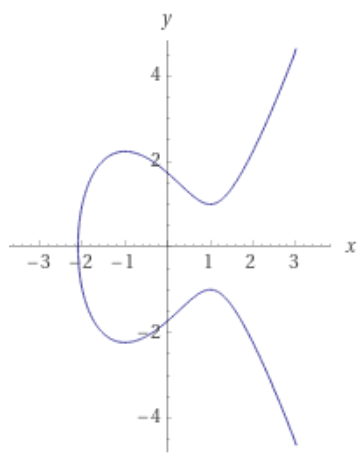
\includegraphics[width=0.5\textwidth]{grafiken/kurve_beispiel_1_punktberechnung.png}
    \caption[Zeichnung der elliptischen Kurve]{Zeichnung der elliptischen Kurve \\ Quelle: Wolframalpha}
    \label{fig:kurve_beispiel_1_punktberechnung}
\end{figure}

Nachdem man allgemein geprüft hat, ob es sich bei der besagten Funktion um eine elliptische Kurve handelt, geht es jetzt um die Findung der Lösungen der umgestellten Gleichung, um alle Punkte zu finden. Dafür gibt es mehrere Möglichkeiten. Die Möglichkeiten haben unterschiedliche Zeit- und Rechenkomplexitäten, wodurch sich die Lösungsmöglichkeiten differenzieren lassen. Je nach Anwendungsfall lohnt sich die Implementierung einer anderen Lösung. Im Folgenden sind drei Möglichkeiten zur Berechnung aller Punkte auf elliptischen Kurven aufgezählt:

\begin{itemize}
\item Brute-Force
\item Punktaddition und Punktverdopplung
\item Algorithmischer Brute-Force
\end{itemize}

Neben dieser drei gängigen Methoden werden in der Mathematik und in der Kryptografie auch die Barrett-Reduktion und weiterhin auch eine Methode, bei welcher sich die Symmetrie zur x-Achse der elliptischen Kurve zur Berechnung zunutze gemacht wird, genutzt. Um diese soll es jedoch nicht gehen. In den folgenden zwei Unterkapiteln wird die Berechnung der Punkte über Brute-Force mit zwei Methoden sowie über die Punktaddition und -verdopplung erläutert und mittels Beispielen verständlich erklärt.

\subsection{Punktbestimmung: Brute-Force-Methode}\label{sec:brute_force}
Wie bereits erläutert wurde, ist die umgestellte Gleichung der elliptischen Kurve in zwei Variablen folgende:
\begin{center}
$y^{2} =  x^{3}$ + ax + b  $\in \mathbb{F}_{p}$
\end{center}

Da die linke Seite mit $y^{2}$ offensichtlich quadratisch ist, muss am Ende auf beiden Seiten der Gleichung die Quadratwurzel gezogen werden, um die Gleichung zu lösen und im weiteren Sinne Punkte auf der Kurve zu finden. Da dies umständlich und im endlichen Körper $\mathbb{F}_{p}$ schwer zu realisieren ist, wird die rechte Seite bis zu einem Quadrat aufgelöst. Dafür muss man als erstes alle Punkte x $\in \mathbb{F}_{p}$ bestimmen, für die $x^{3} + ax + b$ ein Quadrat in $\mathbb{F}_{p}$ sind. Die Quadratprüfung ist dabei simpel: Man geht jedes Element in $\mathbb{F}_{p}$ von 0 bis p-1 durch und prüft, ob das quadrierte Element in der Restklasse ein Quadrat ist. Hierbei geht es um keine komplexe Rechnung, sondern lediglich um stupides ausprobieren. Zur Verdeutlichung folgendes Beispiel: Wir haben den Körper $\mathbb{F}_{5}$. Der Körper beinhaltet die Elemente $\mathbb{F}_{5}$ = {0, 1, 2, 3, 4}. Die Quadrate mitsamt ihrer Wurzeln sind folgende:
\begin{center}
$0 = 0^{2} \qquad 1 = 1^{2} = 4^{2} \qquad 4 = 2^{2} = 3^{2}$
\end{center}

Die Zahlen 0, 1 und 4 sind demnach in $\mathbb{F}_{5}$ Quadrate. Die Wurzeln wurden der Vollständigkeit halber ebenfalls obig rechts des Quadrates notiert. Man berechnet die Quadrate nach folgendem Schema:

\begin{enumerate}
\item Man hat k mit k $\in \mathbb{F}_{p}$
\item Man beginnt bei k = 0
\item Es wird quadriert mit $k^{2}$
\item Der Wert von $k^{2}$ in $\mathbb{F}_{p}$ wird ermittelt, dafür rechnet man $k^{2}$ mod(p)
\item Die ermittelte Zahl ist ein Quadrat in $\mathbb{F}_{p}$
\item Man wiederholt alle Schritte mit allen k von 0 bis p-1
\item Am Ende hat man alle Quadrate und ihre zugehörigen Wurzeln
\end{enumerate}

Dies wird anhand eines ausführlichen Beispiels deutlich. Sei p = 11 und somit $\mathbb{F}_{p}$ = $\mathbb{F}_{11}$. 

\begin{itemize}
\item $0^{2} \equiv 0 $  mod(11)
\item $1^{2} \equiv 1 $  mod(11)
\item $2^{2} \equiv 4 $  mod(11)
\item $3^{2} \equiv 9 $  mod(11)
\item $4^{2} \equiv 5 $  mod(11)
\item $5^{2} \equiv 3 $  mod(11)
\item $6^{2} \equiv 3 $  mod(11)
\item $7^{2} \equiv 5 $  mod(11)
\item $8^{2} \equiv 9 $  mod(11)
\item $9^{2} \equiv 4 $  mod(11)
\item $10^{2} \equiv 1 $  mod(11)
\end{itemize}

Wenn man die Null dazuzählt, hat $\mathbb{F}_{11}$ die Quadrate 0, 1, 3, 4, 5, 9. Im Folgenden sind die Quadrate mitsamt ihrer Wurzeln aufgeschrieben:

\begin{itemize}
\item Quadrat: 0 $\quad$ Wurzel 1: $0$
\item Quadrat: 1 $\quad$ Wurzel 1: $1 \quad$ Wurzel 2: $10$
\item Quadrat: 3 $\quad$ Wurzel 1: $5 \quad$ Wurzel 2: $6$
\item Quadrat: 4 $\quad$ Wurzel 1: $2 \quad$ Wurzel 2: $9$
\item Quadrat: 5 $\quad$ Wurzel 1: $4 \quad$ Wurzel 2: $7$
\item Quadrat: 9 $\quad$ Wurzel 1: $3 \quad$ Wurzel 2: $8$
\end{itemize}

Die berechneten Quadrate und Wurzeln sind nötig, um die Punkte zu bestimmen. Um dies zu bewerkstelligen, wird die Gleichung der elliptischen Kurve in zwei Variablen benötigt. Um die benötigte Formel zu erhalten, überführen wir die Ausgangsgleichung in zwei Variablen in eine Funktionsgleichung mit einer Variablen:
\begin{center}
$y^{2} =  x^{3}$ + ax + b  $\in \mathbb{F}_{p} \qquad \Longrightarrow \qquad f(x) =  x^{3}$ + ax + b  $\in \mathbb{F}_{p}$
\end{center}

Diese Funktionsgleichung ist der Ausgangspunkt für die Berechnung der Punkte. Man setzt nun alle x-Werte von 0 bis p-1 in die Funktionsgleichung ein. Jene x-Werte, welche die Quadrate ergeben, werden für die Punktbestimmung benötigt. Nehme als Beispiel p = 11. Wir haben die Quadrate und die Wurzeln oben bereits ausgerechnet. Sei weiterhin die Gleichung einer elliptischen Kurve E gegeben durch
\begin{center}
$F(X, Y) =  Y^{2} - X^{3} + 10 \cdot X + 8 \in \mathbb{F}_{11}$
\end{center}

Damit ist die umgestellte Gleichung in zwei Variablen und die Funktionsgleichung mit einer Variablen
\begin{center}
$y^{2} =  x^{3}$ + x + 3 $\qquad \Longrightarrow \qquad f(x) =  x^{3}$ + x + 3 $\in \mathbb{F}_{11}$
\end{center}
Setzen wir nun alle Elemente von 0 bis p-1 in die Funktionsgleichung ein und betrachten die Ergebnisse:

\begin{itemize}
\item $f(0) =  0^{3}$ + 0 + 3 = 3 $\in \mathbb{F}_{11} \qquad \Longrightarrow \qquad$ Quadrat
\item $f(1) =  1^{3}$ + 1 + 3 = 5 $\in \mathbb{F}_{11} \qquad \Longrightarrow \qquad$ Quadrat
\item $f(2) =  2^{3}$ + 2 + 3 = 2 $\in \mathbb{F}_{11}$
\item $f(3) =  3^{3}$ + 3 + 3 = 0 $\in \mathbb{F}_{11} \qquad \Longrightarrow \qquad$ Quadrat
\item $f(4) =  4^{3}$ + 4 + 3 = 5 $\in \mathbb{F}_{11} \qquad \Longrightarrow \qquad$ Quadrat
\item $f(5) =  5^{3}$ + 5 + 3 = 1 $\in \mathbb{F}_{11} \qquad \Longrightarrow \qquad$ Quadrat
\item $f(6) =  6^{3}$ + 6 + 3 = 5 $\in \mathbb{F}_{11} \qquad \Longrightarrow \qquad$ Quadrat
\item $f(7) =  7^{3}$ + 7 + 3 = 1 $\in \mathbb{F}_{11} \qquad \Longrightarrow \qquad$ Quadrat
\item $f(8) =  8^{3}$ + 8 + 3 = 6 $\in \mathbb{F}_{11}$
\item $f(9) =  9^{3}$ + 9 + 3 = 4 $\in \mathbb{F}_{11} \qquad \Longrightarrow \qquad$ Quadrat
\item $f(10) = 10^{3}$ + 10 + 3 = 1 $\in \mathbb{F}_{11} \qquad \Longrightarrow \qquad$ Quadrat
\end{itemize}

Die Ergebnisse zeigen dass für die folgenden $x$-Werte $f(x)$ ein Quadrat ist: 0, 1, 3, 4, 5, 6, 7, 9, 10. Bis jetzt wurde der einfache Brute-Force durchgeführt. Man muss nur noch wenige Schritte durchführen, um die Punkte auf der elliptischen Kurve zu bestimmen. Wir haben jetzt die Quadrate, die dazugehörigen Wurzeln sowie die x-Werte, welche Quadrate sind. Wie kombiniert man diese, um die Punkte auf der elliptischen Kurve zu erhalten? Es gilt, die Informationen der Punkte P mit P = (x, y) der elliptischen Kurve zu erhalten. Für den x-Wert der Punkte nimmt man das Ergebnis des eingesetzten x von 0 bis p-1 in die Funktion. Man nimmt als x-Wert das vorhandene Quadrat. Die y-Werte der Punkte ergeben sich aus dem Ergebnis des eingesetzten x in die umgestellte Funktion mit einer Variablen. Man nimmt die Wurzeln des zugehörigen Quadrates zum Ergebnis. Daraus ergeben sich die folgenden Punkte auf der obig eingeführten elliptischen Kurve E:

\begin{itemize}
\item $f(0) = 3 \quad \Longrightarrow \quad$ Punkt 1: $(0, 5) \quad$ Punkt 2: $(0, 6)$
\item $f(1) = 5 \quad \Longrightarrow \quad$ Punkt 1: $(1, 4) \quad$ Punkt 2: $(1, 7)$
\item $f(3) = 0 \quad \Longrightarrow \quad$ Punkt 1: $(3, 0)$
\item $f(4) = 5 \quad \Longrightarrow \quad$ Punkt 1: $(4, 4) \quad$ Punkt 2: $(4, 7)$
\item $f(5) = 1 \quad \Longrightarrow \quad$ Punkt 1: $(5, 1) \quad$ Punkt 2: $(5, 10)$
\item $f(6) = 5 \quad \Longrightarrow \quad$ Punkt 1: $(6, 4) \quad$ Punkt 2: $(6, 7)$
\item $f(7) = 1 \quad \Longrightarrow \quad$ Punkt 1: $(7, 1) \quad$ Punkt 2: $(7, 10)$
\item $f(9) = 4 \quad \Longrightarrow \quad$ Punkt 1: $(9, 2) \quad$ Punkt 2: $(9, 9)$
\item $f(10) = 1 \quad \Longrightarrow \quad$ Punkt 1: $(10, 1) \quad$ Punkt 2: $(10, 10)$
\end{itemize}

Die Berechnung der Punkte über die Brute-Force-Methode ist sehr umständlich. Insbesondere, wenn das gewählte p groß ist, dann ist diese Brute-Force-Methode sehr aufwendig. Es müssen alle Quadrate in $\mathbb{F}_{p}$ und deren zugehörigen Wurzeln berechnet werden. Weiterhin entsteht Zeit- und Rechenaufwand beim Einsetzen in die Funktionen. In der Kryptografie ist jedoch die Wahl besonders großer p gängig, um ein hohes Sicherheitsniveau zu erreichen. Aus diesem Grund werden im Folgenden die beiden anderen angeführten Lösungsmöglichkeiten angeführt. 

\subsection{Punktbestimmung: Punktaddition und -verdopplung}
Eine weitere Methode zur Berechnung von Punkten auf einer elliptischen Kurve ist die Punktaddition und die Punktverdopplung. Dies ist eine elegante Methode, da man über einen simplen Algorithmus alle Punkte auf einer elliptischen Kurve bestimmen kann, sofern der Startpunkt ein primitives Element der elliptischen Kurve ist. Der Nachteil dieser Methode ist jedoch, dass im Vorfeld ein Punkt auf der elliptischen Kurve bekannt sein muss, der gleichzeitig ein Erzeuger der Gruppe ist oder eine hohe Ordnung auf der Kurve hat. Dieser Punkt muss über die Brute-Force-Methode oder einem anderen Ansatz berechnet werden oder ein ist im Voraus bekannt. Die offene Frage ist jedoch, ob jeder beliebige Punkt als Ausgangsobjekt genutzt werden kann, um auf seiner Grundlage alle anderen Punkte zu erzeugen.\\

Um dies herauszufinden, müssen noch einmal die Gruppeneigenschaften von elliptischen Kurven über $\mathbb{F}_{p}$ betrachtet werden. Hankerson, Menezes und Vanstone beschreiben in ihrem Buch \glqq\textit{Guide to Elliptic Curve Cryptography}\grqq diese Gruppeneigenschaften und erklären damit, wie man herausfindet, ob es sich um eine zyklische Gruppe handelt und damit in welterem Sinne, welche Punkte auf der elliptischen Kurve Generatoren sind \cite[vgl.][S. 82-84]{Hankerson2004}. Sei E eine elliptische Kurve über $\mathbb{F}_{p}$. Die Anzahl der Punkte in E($\mathbb{F}_{p}$), bezeichnet als
$\overline{E}(\mathbb{F}_{p})$, wird als die Ordnung von E über $\mathbb{F}_{p}$ bezeichnet. Dabei ist der imaginäre Punkt im Unendlichen inkludiert. Im Folgenden ist es wichtig herauszufinden, ob E eine zyklische Gruppe ist. Eine elliptische Kurve E über $\mathbb{F}_{p}$ ist eine zyklische Gruppe, wenn $\overline{E}(\mathbb{F}_{p})$ eine Primzahl ist. Dabei gilt die Regel: Definiert $\overline{E}(\mathbb{F}_{p})$ eine zyklische Gruppe, so ist die Anzahl der Punkte der Kurve mit hoher Wahrscheinlichkeit eine Primzahl. Dadurch ergibt sich ein Vorteil. Wenn die Anzahl der Punkte prim ist, dann sagt das Lagrange Theorem aus, dass jeder Punkt auf der Kurve ein Erzeuger der Gruppe ist. Dadurch kann aus jedem Punkt alle anderen Punkte berechnet werden. Um dies weiter auszuführen, wird die bereits angeführte Hasse-Weil-Schranke genutzt, um eine Abschätzung über die Anzahl der Punkte abzugeben.
\begin{center}
$p + 1 - 2 \cdot \sqrt{p} \leq | \overline{E} | \leq p + 1 + 2 \cdot \sqrt{p}$
\end{center} 

Diese gibt eine obere und untere Schranke für $\overline{E}$ an. Liegt innerhalb dieser Schranke eine Primzahl, so ist die Wahrscheinlichkeit dafür, dass E eine zyklische Gruppe über $\mathbb{F}_{p}$ definiert, sehr hoch. Ist eine elliptische Kurve E eine zyklische Gruppe und die Anzahl der Punkte ist nicht prim, dann hat sie mindestens ein Element, welches ein Erzeuger der Gruppe ist. Mit diesem Erzeugerelement lassen sich alle anderen Elemente der Gruppe durch Punktverdopplung bzw. Punktaddition generieren. Der Punkt hat damit die gleiche Ordnung wie E. Ist der Erzeuger und ein weiterer Punkt gegeben, so lassen sich auch über die Punktaddition weitere Punkte finden. Weiterhin sei gesagt, dass der Punkt im Unendlichen kein Erzeuger sein kann. Die Berechnung aller Punkte auf der Kurve ist trivial, wenn der Erzeuger bekannt ist. Nehmen wir als Beispiel eine elliptische Kurve E gegeben durch
\begin{center}
$y^{2} =  x^{3} + 2x + 2 \in \mathbb{F}_{17}$
\end{center}

Der Erzeuger der Gruppe ist der Punkt P = (5, 1). Um zu zeigen, dass dieser Punkt ein Erzeuger oder Generator ist, muss er mit sich selbst so oft addiert werden, bis er den Punkt im Unendlichen ergibt. Bei dem gegebenen Punkt ist dies bei 19 $\cdot$ P der Fall. Gegeben sei außerdem 18 $\cdot$ P = (5, -1). Da 19 $\cdot$ P = 18 $\cdot$ P + P = (5, 1) + (5, -1) = $\mathcal O$. Dieses kurze Beispiel macht deutlich, dass es aufwendig sein kann zu prüfen, ob ein Punkt P ein Erzeuger ist. In der Praxis werden in Kryptosystemen Punktgeneratoren mit großer Ordnung gewählt, um die Sicherheit in den verwendeten kryptografischen System zu gewährleisten. Der Erzeuger der Gruppe ist so nicht einfach berechenbar. In den folgenden Beispielen ist jedoch ein Erzeuger gegeben, damit die Punktaddition respektive die Punkterdopplung trivial ist.\\

Bevor das Beispiel durchgegangen wird, werden noch einmal die benötigten Formeln und die Vorgehensweise erläutert. Es sei ein Erzeugerpunkt P gegeben mit $P = (x_1, y_2)$. Da nur dieser gegeben ist, wird er mit sich selbst addiert. Somit gilt: 2 $\cdot$ P = P + P. Durch die Punktverdopplung entsteht ein neuer Punkt. P kann jetzt mit 2 $\cdot$ P addiert werden. Dies wird solange fortgeführt, bis der Punkt im Unendlichen herauskommt. Anschließend hat man alle Punkte auf E berechnet. Im Folgenden wird die Vorgehensweise über Pseudocode in Python erläutert, wenn ein Erzeugerpunkt gegeben ist. Es soll gesagt sein, dass es sich hierbei um eine starke Vereinfachung handelt. Beispielsweise wird nicht darauf eingegangen, dass das p des Primkörpers für die Durchführung der Addition von Punkten benötigt wird:\\

\begin{lstlisting}[caption={Punktberechnung in Python}, captionpos=b]
function punktbestimmung(P, Q):
	Punkte = []	
	if P = UNENDLICH:
		return FEHLER		
	zaehler = 0
	while 1:
		if P = Q
			Punkte[zaehler] = P + P
			Q = Punkte[zaehler]
			if Q = UNENDLICH
			zaehler = zaehler + 1	
		if P != Q
			Punkte[zaehler] = P + Q
			Q = Punkte[zaehler]
			if Q = UNENDLICH
			zaehler = zaehler + 1
	return Punkte
\end{lstlisting}

Der Pseudocode zeigt lediglich eine beispielhafte Umsetzung. In \ref{sec:python_add_double} wird der ausprogrammierte Python-Code inklusive Erklärungen angegeben und weiter ausgeführt.\\

Damit die Theorie anschaulich wird, folgt nun ein Beispiel für die Punktaddition und -verdopplung, um alle Punkte auf einer elliptischen Kurve zu berechnen. Das Beispiel ist angelehnt an \cite[vgl.][S. 279-280]{Paar.2016}. Gegeben sei eine elliptische Kurve E mit
\begin{center}
$y^{2} =  x^{3} + 2x + 2 \in \mathbb{F}_{17}$
\end{center}

Weiterhin sei ein Punkt P auf der elliptischen Kurve gegeben durch P = (5, 1). Da nur ein Punkt gegeben ist, muss dieser verdoppelt werden. Es gilt $2 \cdot P = P + P = (x_1, y_1) + (x_2, y_2) = (5, 1) + (5, 1) = (x_3, y_3)$. Es gilt
$$s = \frac{3x_1^2 + a}{2y_1} \text{, da } P = Q $$
Setzt man die Werte ein, erhält man 
$$s = \frac{3x_1^2 + a}{2y_1} = (2 \cdot 1)^{-1}(3 \cdot 5^2 + 2) = 2^{-1} \cdot 9 \equiv 9 \cdot 9 \equiv 13 \text{ mod } 17$$
Da nun s berechnet wurde, kann man nun die folgenden Formeln lösen und $x_3$ sowie $y_3$ bestimmen.
$$x_3 = s^2 - x_1 - x_2 = 13^2 - 5 - 5 = 159 \equiv 6 \text{ mod } 17$$
$$y_3 = s(x_1 - x_3) - y_1 = 13(5 - 6) - 1 = - 14 \equiv 3 \text{ mod } 17$$
Damit ist $2 \cdot P = (6, 3)$. Da jetzt zwei (unterschiedliche) Punkte vorhanden sind, kann nun die im Vergleich zur Punktverdopplung simplere Punktaddition durchgeführt werden, um weitere Punkte zu finden. Dafür addieren wir nun alle aufeinander folgenden Punkte zusammen. $3 \cdot P = P + Q = (5, 1) + (6, 3)$, wobei Q = $2 \cdot P$.\\
Für s berechnet man
$$s = \frac{y_2 - y_1}{x_2 - x_1} \text{, da } P \neq Q $$
Daraus ergibt sich 
$$s = \frac{y_2 - y_1}{x_2 -x_1} = \frac{3 - 1}{6 - 5} = 2 \text{ mod } 17$$
$$x_3 = s^2 - x_1 - x_2 = 4 - 5 - 6 = - 7 \equiv 10 \text{ mod } 17$$
$$y_3 = s(x_1 - x_3) - y_1 = 2(5 - 10) - 1 = - 11 \equiv 6 \text{ mod } 17$$
Damit ist $3 \cdot P = (10, 6)$. $4 \cdot P = P + Q = (5, 1) + (10, 6)$, wobei Q = $3 \cdot P$. 
Daraus ergibt sich 
$$s = \frac{y_2 - y_1}{x_2 -x_1} = \frac{6 - 1}{10 - 5} = 1 \text{ mod } 17$$
$$x_3 = s^2 - x_1 - x_2 = 1 - 5 - 10 = -14 \equiv 3 \text{ mod } 17$$
$$y_3 = s(x_1 - x_3) - y_1 = 1(5 - 3) - 1 = 1 \text{ mod } 17$$
Damit ist $4 \cdot P = (3, 1)$. $5 \cdot P = P + Q = (5, 1) + (3, 1)$, wobei Q = $4 \cdot P$.\\
Daraus ergibt sich 
$$s = \frac{y_2 - y_1}{x_2 -x_1} = \frac{1 - 1}{3 - 5} = 0 \text{ mod } 17$$
$$x_3 = s^2 - x_1 - x_2 = 0 - 5 - 3 = - 8 \equiv 9 \text{ mod } 17$$
$$y_3 = s(x_1 - x_3) - y_1 = 0(5 - 9) - 1 = - 1 \equiv 16 \text{ mod } 17$$
Damit ist $5 \cdot P = (9, 16)$. $6 \cdot P = P + Q = (5, 1) + (9, 16)$, wobei Q = $5 \cdot P$.\\
Daraus ergibt sich 
$$s = \frac{y_2 - y_1}{x_2 -x_1} = \frac{16 - 1}{9 - 5} = 15 \cdot 13 \equiv 8 \text{ mod } 17$$
$$x_3 = s^2 - x_1 - x_2 = 13 - 5 - 9 = -1 \equiv 16 \text{ mod } 17$$
$$y_3 = s(x_1 - x_3) - y_1 = 8(5 - 16) - 1 = - 89 \equiv 13 \text{ mod } 17$$
Damit ist $6 \cdot P = (16, 13)$. $7 \cdot P = P + Q = (5, 1) + (16, 13)$, wobei Q = $6 \cdot P$.\\
Daraus ergibt sich 
$$s = \frac{y_2 - y_1}{x_2 -x_1} = \frac{13 - 1}{16 - 5} = 12 \cdot 14 \equiv 15 \text{ mod } 17$$
$$x_3 = s^2 - x_1 - x_2 = 4 - 5 - 16 = - 17 \equiv 0 \text{ mod } 17$$
$$y_3 = s(x_1 - x_3) - y_1 = 15(5 - 0) - 1 = 6 \text{ mod } 17$$
Damit ist $7 \cdot P = (0, 6)$. $8 \cdot P = P + Q = (5, 1) + (0, 6)$, wobei Q = $7 \cdot P$.\\
Daraus ergibt sich 
$$s = \frac{y_2 - y_1}{x_2 -x_1} = \frac{6 - 1}{0 - 5} = -1 \equiv 16 \text{ mod } 17$$
$$x_3 = s^2 - x_1 - x_2 = 1 - 5 - 0 = -4 \equiv 13 \text{ mod } 17$$
$$y_3 = s(x_1 - x_3) - y_1 = 16(5 - 13) - 1 = - 129 \equiv 7 \text{ mod } 17$$
Damit ist $8 \cdot P = (13, 7)$. $9 \cdot P = P + Q = (5, 1) + (13, 7)$, wobei Q = $8 \cdot P$.\\
Daraus ergibt sich 
$$s = \frac{y_2 - y_1}{x_2 -x_1} = \frac{7 - 1}{13 - 5} = 6 \cdot 15 = 5 \text{ mod } 17$$
$$x_3 = s^2 - x_1 - x_2 = 25 - 5 - 13 = 7 \text{ mod } 17$$
$$y_3 = s(x_1 - x_3) - y_1 = 5(5 - 7) - 1 = - 11 \equiv 6 \text{ mod } 17$$
Damit ist $9 \cdot P = (7, 6)$. $10 \cdot P = P + Q = (5, 1) + (7, 6)$, wobei Q = $9 \cdot P$.\\
Daraus ergibt sich 
$$s = \frac{y_2 - y_1}{x_2 -x_1} = \frac{6 - 1}{7 - 5} = 5 \cdot 9 \equiv 11 \text{ mod } 17$$
$$x_3 = s^2 - x_1 - x_2 = 2 - 5 - 7 = -10 \equiv 7 \text{ mod } 17$$
$$y_3 = s(x_1 - x_3) - y_1 = 11(5 - 7) - 1 = - 23 \equiv 11 \text{ mod } 17$$
Damit ist $10 \cdot P = (7, 11)$. $11 \cdot P = P + Q = (5, 1) + (7, 11)$, wobei Q = $10 \cdot P$.\\
Daraus ergibt sich 
$$s = \frac{y_2 - y_1}{x_2 -x_1} = \frac{11 - 1}{7 - 5} = 5 \text{ mod } 17$$
$$x_3 = s^2 - x_1 - x_2 = 25 - 5 - 7 = 13 \text{ mod } 17$$
$$y_3 = s(x_1 - x_3) - y_1 = 5(5 - 13) - 1 = - 41 \equiv 10 \text{ mod } 17$$
Damit ist $11 \cdot P = (13, 10)$. $12 \cdot P = P + Q = (5, 1) + (13, 10)$, wobei Q = $11 \cdot P$.\\
Daraus ergibt sich 
$$s = \frac{y_2 - y_1}{x_2 -x_1} = \frac{10 - 1}{13 - 5} = 9 \cdot 15 \equiv 16 \text{ mod } 17$$
$$x_3 = s^2 - x_1 - x_2 = 1 - 5 - 13 = - 17 \equiv 0 \text{ mod } 17$$
$$y_3 = s(x_1 - x_3) - y_1 = 16(5 - 0) - 1 = 79 \equiv 11 \text{ mod } 17$$
Damit ist $12 \cdot P = (0, 11)$. $13 \cdot P = P + Q = (5, 1) + (0, 11)$, wobei Q = $12 \cdot P$.\\
Daraus ergibt sich 
$$s = \frac{y_2 - y_1}{x_2 -x_1} = \frac{11 - 1}{0 - 5} = - 2 \equiv 15 \text{ mod } 17$$
$$x_3 = s^2 - x_1 - x_2 = 4 - 5 - 0 = - 1 \equiv 16 \text{ mod } 17$$
$$y_3 = s(x_1 - x_3) - y_1 = 15(5 - 16) - 1 = - 166 \equiv 4 \text{ mod } 17$$
Damit ist $13 \cdot P = (16, 4)$. $14 \cdot P = P + Q = (5, 1) + (16, 4)$, wobei Q = $13 \cdot P$.\\
Daraus ergibt sich 
$$s = \frac{y_2 - y_1}{x_2 -x_1} = \frac{4 - 1}{16 - 5} = 3 \cdot 14 \equiv 8 \text{ mod } 17$$
$$x_3 = s^2 - x_1 - x_2 = 13 - 5 - 16 = - 8 \equiv 9 \text{ mod } 17$$
$$y_3 = s(x_1 - x_3) - y_1 = 8(5 - 9) - 1 = - 33 \equiv 1 \text{ mod } 17$$
Damit ist $14 \cdot P = (9, 1)$. $15 \cdot P = P + Q = (5, 1) + (9, 1)$, wobei Q = $14 \cdot P$.\\
Daraus ergibt sich 
$$s = \frac{y_2 - y_1}{x_2 -x_1} = \frac{1 - 1}{9 - 5} = 0 \text{ mod } 17$$
$$x_3 = s^2 - x_1 - x_2 = 0 - 5 - 9 = - 14 \equiv 3 \text{ mod } 17$$
$$y_3 = s(x_1 - x_3) - y_1 = 0(5 - 3) - 1 = - 1 \equiv 16 \text{ mod } 17$$
Damit ist $15 \cdot P = (3, 16)$. $16 \cdot P = P + Q = (5, 1) + (3, 16)$, wobei Q = $15 \cdot P$.\\
Daraus ergibt sich 
$$s = \frac{y_2 - y_1}{x_2 -x_1} = \frac{16 - 1}{3 - 5} = - 15 \cdot 9 \equiv 1 \text{ mod } 17$$
$$x_3 = s^2 - x_1 - x_2 = 1 - 5 - 3 = - 7 \equiv 10 \text{ mod } 17$$
$$y_3 = s(x_1 - x_3) - y_1 = 1(5 - 10) - 1 = - 6 \equiv 11 \text{ mod } 17$$
Damit ist $16 \cdot P = (10, 11)$. $17 \cdot P = P + Q = (5, 1) + (10, 11)$, wobei Q = $16 \cdot P$.\\
Daraus ergibt sich 
$$s = \frac{y_2 - y_1}{x_2 -x_1} = \frac{11 - 1}{10 - 5} = 2 \text{ mod } 17$$
$$x_3 = s^2 - x_1 - x_2 = 4 - 5 - 10 = - 11 \equiv 6 \text{ mod } 17$$
$$y_3 = s(x_1 - x_3) - y_1 = 2(5 - 6) - 1 = - 3 \equiv 14 \text{ mod } 17$$
Damit ist $17 \cdot P = (6, 14)$. $18 \cdot P = P + Q = (5, 1) + (6, 14)$, wobei Q = $17 \cdot P$.\\
Daraus ergibt sich 
$$s = \frac{y_2 - y_1}{x_2 -x_1} = \frac{14 - 1}{6 - 5} = 13 \text{ mod } 17$$
$$x_3 = s^2 - x_1 - x_2 = 16 - 5 - 6 = 5 \text{ mod } 17$$
$$y_3 = s(x_1 - x_3) - y_1 = 13(5 - 5) - 1 = - 1 \equiv 16 \text{ mod } 17$$
Damit ist $18 \cdot P = (5, 16)$. $19 \cdot P = P + Q = (5, 1) + (5, 16) = \infty $, wobei Q = $18 \cdot P$. Der Punkt im unendlichen wurde erreicht, womit nun alle Punkte gefunden wurden. Da die Ordnung der Untergruppe von P auf der elliptischen Kurve ein Teiler der Gruppenordnung ist, muss die Anzahl der Elemente der Kurve ein Vielfaches von 19 sein. Da wir insgesamt 19 Punkte mit dem Punkt im Unendlichen berechnet haben und $2 \cdot 19$ zu groß für die Hasse-Weil-Schranke ist da es das Intervall überschreitet, beudeutet dies, dass alle Punkte auf der elliptischen Kurve gefunden wurden.\\

Ähnlich wie bei der Brute-Force-Methode in \ref{sec:brute_force} ist die Berechnung über die Punktaddition und -verdopplung sehr rechenaufwendig. Die Schritte können in dieser Methode nicht ohne weiteres vereinfacht werden. Dadurch bleiben nur die Möglichkeiten offen, diese Methode in Code abzubilden, wie in \ref{sec:python_add_double} oder es händisch auszurechnen, was sehr zeit- und rechenaufwendig ist. Berechnet man die Punkte mit der Hand, dann ist die Fehleranfälligkeit hoch, da die vielen Rechnungen schnell unübersichtlich werden. Dadurch bleibt die Implementierung dieser Methode über Programmcode die einzige logische und effiziente Möglichkeit. Die nächste angeführte Methode zur Berechnung von Punkten auf einer elliptischen Kurve ist die algorithmische Brute-Force-Methode. Durch sie kann im Vergleich zu den zwei vorausgehenden Methoden der Zeit- und Rechenaufwand verringert werden.

\subsection{Punktbestimmung: Algorithmische Brute-Force-Methode}
Die algorithmische Brute-Force-Methode ist der klassischen Brute-Force-Methode in \ref{sec:brute_force} sehr ähnlich. Sie unterscheidet sich jedoch in einem wichtigen Aspelt. Während man bei der klassichen Methode die Quadrate und ihre Quadratwurzeln durch Ausprobieren aller Möglichkeiten herausfindet, wird bei der algorithmischen Methode die Findung der Quadrate und ihrer Wurzeln über einen Algorithmus durchgeführt. Der Algorithmus beinhaltet eine Quadratprüfung sowie eine Quadratwurzelprüfung über Schlussfolgerungen aus dem Satz von Fermat. Bei großen $p$ ist das Finden von Quadraten und der Quadratwurzeln sehr aufwendig. Der Vorteil der algorithmischen Methode ist, dass diese auch bei einem großen $p$ noch effizient berechnet werden können. 

\paragraph{Satz von Fermat}
Ist $\mathbb{F}_q$ ein endlicher Körper mit $q = p^e$ Elementen und p ist eine Primzahl, so ist die Einheitengruppe $\mathbb{F}_q^* = \mathbb{F}_q \setminus \{0\}$ zyklisch von der Ordnung $q - 1$.

Aus diesem Satz lassen sich zwei Folgerungen herleiten, welche Grundlage für die algorithmische Brute-Force-Methode sind. Die genaue Herleitung der Folgerungen soll kein Teil dieser Arbeit sein. Die Folgerungen wurden dem Script von Hübl entnommen \cite[vgl.][S. 269]{reinholdhuebl}.

\paragraph{Folgerung 1}
Ist $\mathbb{F}_p$ ein endlicher Primkörper mit einer Primzahl $p \geq 3$, so ist ein $x \in \mathbb{F}_p^*$ genau dann ein Quadrat, wenn $x^{\frac{p - 1}{2}} = 1$. Genau die Hälfte der Elemente von $\mathbb{F}_p^*$ sind Quadrate.

\paragraph{Folgerung 2}
Ist p eine Primzahl, für die 4 ein Teiler von $p + 1$ ist und ist $x \in \mathbb{F}_p^*$ ein Quadrat, so ist $$a = x^{\frac{p + 1}{4}}$$ eine Quadratwurzel von $x$.\\

Dies wird nun an einem Beispiel verdeutlicht. Gegeben sei ein Polynom einer elliptischen Kurve E der Form $$F(X, Y) = Y^{2} - X^{3} - X - 1 \in \mathbb{F}_{7}$$ Stellt man die Gleichung der Funktion nach $y^{2}$ um, dann erhält man folgende Gleichung: $$y^{2} =  x^{3} + x + 1 \text{ mod }7$$

Um nun zu prüfen, welche Elemente in $\mathbb{F}_{7}$ Quadrate sind, muss für jedes Element geprüft werden, ob $x^{\frac{p - 1}{2}} = 1$ in $\mathbb{F}_{7}$.\\

\begin{itemize}
\item $1^{\frac{7 - 1}{2}} = 1$ mod(7)
\item $2^{\frac{7 - 1}{2}} = 1$ mod(7)
\item $3^{\frac{7 - 1}{2}} = 6 \neq 1$ mod(7)
\item $4^{\frac{7 - 1}{2}} = 1$ mod(7)
\item $5^{\frac{7 - 1}{2}} = 6 \neq 1$ mod(7)
\item $6^{\frac{7 - 1}{2}} = 6 \neq 1$ mod(7)
\end{itemize} 

Die Kandidaten für Quadrate auf der Kurve sind die 1, die 2 und die 4. Hier erkennt man auch, dass genau die Hälfte der Elemente Quadrate sind. Im Folgenden werden die Kandidaten in die umgestellte Gleichung eingesetzt.

\begin{itemize}
\item $f(0) =  0^{3}$ + 0 + 1 = 1 $\in \mathbb{F}_{7} \qquad \Longrightarrow \qquad$ Quadrat
\item $f(1) =  1^{3}$ + 1 + 1 = 3 $\in \mathbb{F}_{7}$
\item $f(2) =  2^{3}$ + 2 + 1 = 4 $\in \mathbb{F}_{7} \qquad \Longrightarrow \qquad$ Quadrat
\item $f(3) =  3^{3}$ + 3 + 1 = 3 $\in \mathbb{F}_{7}$
\item $f(4) =  4^{3}$ + 4 + 1 = 6 $\in \mathbb{F}_{7}$
\item $f(5) =  5^{3}$ + 5 + 1 = 5 $\in \mathbb{F}_{7}$
\item $f(6) =  6^{3}$ + 6 + 1 = 6 $\in \mathbb{F}_{7}$
\end{itemize}

Daraus ergeben sich die folgenden Punkte auf der elliptischen Kurve E:

\begin{itemize}
\item $f(0) = 1 \quad \Longrightarrow \quad$ Punkt 1: $(0, 1) \quad$ Punkt 2: $(0, 6)$
\item $f(2) = 4 \quad \Longrightarrow \quad$ Punkt 1: $(2, 2) \quad$ Punkt 2: $(2, 5)$
\end{itemize}

wie man sieht, ist die Anwendung relativ einfach umzusetzen. Es gibt jedoch einen weiteren Fall, welcher betrachtet werden muss, um die Quadrate zu finden. Der Fall 1 wurde soeben betrachtet und anhand eines beispiels durchgerechnet. In diesem Fall ist 4 ein Teiler von $p + 1$ ist. Wenn es diesen Fall gibt kann es auch sein, dass $4 \hspace{-0.4em}\not\hspace{0.025em}|\, (p + 1)$ ist. Für diesen Fall 2 gibt es einen probabilistischen Ansatz, um die Quadratwurzeln zu finden. Dafür wird eine Induktion durchgeführt.\\

XXXXX\\

XXXXX\\

Hübl beschreibt in seinem Script die allgemeine Vorgehensweise für den algorithmischen Brute-Force \cite[vgl.][S. 270-272]{reinholdhuebl}. Gegeben sei ein $x \in \mathbb{F}_p^*$.

\begin{enumerate}
\item Berechne $x^{\frac{p - 1}{2}}$ in $\mathbb{F}_p$. Falls $x^{\frac{p - 1}{2}} \neq 1$: \textbf{STOPP}, x ist kein Quadrat in $\mathbb{F}_p$.
\item Falls $4 | (p + 1)$, so setze $$a =  x^{\frac{p + 1}{4}}$$ Falls $4 \hspace{-0.4em}\not\hspace{0.025em}|\, (p + 1)$, wähle ein $b in \mathbb{F}_p$ mit $b^{\frac{p - 1}{2}} = -1$, schreibe $\frac{p - 1}{2} = 2^l \cdot t$ wie oben und konstruiere $$a =  x^{\frac{t + 1}{2}} \cdot b^n$$ wie oben.
\item Die Zahl $a$ ist eine Quadratwurzel von x in $\mathbb{F}_p$.
\end{enumerate}


\section{Diskreter Logarithmusproblem über elliptischen Kurven} \label{sec:DLPüberEC}
Wie in Kapitel XY gezeigt, kann das DLP verallgemeinert werden, sodass über jeder zyklischen Gruppe (mehr oder weniger effektiv) ein DLP definiert erden kann. Im ersten Abschnitts dieses Kapitels wurden die Gruppeneigenschaften der Punktmenge auf der elliptischen Kurve gezeigt. Gruppenelemente werden können über die Gruppenoperation $+$ \textit{addiert} werden. Es gilt der Folgende Satz:

\paragraph{Satz:}
Die Punkte einer elliptischen Kurve zusammen mit $O$ haben zyklischen Untergruppen. Unter bestimmten Bedingungen bilden \textit{alle} Punkte einer elliptischen Kurve eine zyklische Gruppe.\\

Um eine kryptografisch \textit{sicheres} DLP zu konstruieren, ist es wichtig die Gruppenkardinalität zu kennen. Deren exakte Bestimmung ist bei elliptischen Kurven jedoch sehr aufwendig. Für die grobe Bestimmung der Gruppenkardinalität wurde in Kapitel XY bereits die Hasse-Weil-Schranke vorgestellt. Diese erlaubt es uns die Anzahl der Punkte einer elliptischen Kurve abzuschätzen. Vereinfacht kann man sagen das die Anzahl der Punkte in etwa $p$ entspricht, wenn die elliptische Kurve über $\mathbb{Z}^*_p$ definiert ist.\\

Im folgenden wollen wir das DLP über elliptischen Kurven definieren:

\paragraph{Definition: Das DLP über elliptischen Kurven (ECDLP)}
Gegeben sei eine elliptische Kurve $E$. Wir betrachten ein primitives Element $P$ und ein beliebiges weiteres Element $T$. Das DLP ist die Bestimmung der natürlichen Zahl $d$ zwischen $1 \leq d \leq \#E$, sodass gilt:
$$\underbrace{P + P + \dots + P}_{d-mal} = d P = T$$\\

Die Bestimmung der natürlichen Zahl $d$ ist wie auch schon beim DLP über $\mathbb{Z}^*_p$ nicht trivial. In einem Kryptosystem wäre dementsprechend die natürliche Zahl $d$ der private Schlüssel und das Element $T$ der öffentliche Schlüssel. Anders als beim DLP über Primkörpern, wo beide Schlüssel natürliche Zahlen waren, ist der private Schlüssel $T$ hier ein Punkt der elliptischen Kurve. Der in der obigen Definition verwendete Ausdruck $dP$ wird \textit{Punktmultiplikation} genannt, da man schreiben kann $T = dP$. Es ist jedoch zu beachten das es dafür keine Rechenvorschrift gibt, die Zahl $d$ mit $P$ zu multiplizieren. Der Ausdruck bedeutet lediglich, dass die Gruppenoperation $d$ mal auf $P$ angewendet wird.\\

Der Erzeuger eines Schlüsselpaars muss allerdings nicht einzeln $d$ mal $P$ auf sich selbst addieren, sonder kann sich eines \textit{Tricks} bedienen. Wie beim DLP über dem Primkörper $\mathbb{Z}^*_p$, wo der Square-And-Multiply-Algorithmus zu effizienten Berechnung des öffentlichen Schlüssels verwendet wurde, kann hier der sog. \textit{Double-And-Add-Algorithmus} verwendet werden. Dieser ist von der Idee her zum Square-And-Multiply-Algorithmus identisch, und unterscheidet sich nur durch die angewandten Operationen. Der folgende Code zeigt eine Beispielhafte Implementierung:

\vspace{\baselineskip}
\begin{lstlisting}[caption={Double-And-Add-Algorithmus in Python}, captionpos=b]
def doubble_and_add(kPriv, start_point):
	binary = bin(kPriv)
	binary = binary[3:]
    cur_point = start_point
    for digit in binary:
        # Doubble
	    cur_point = curve.add(cur_point, cur_point)
		if digit == "1":
	        # Add
            cur_point = curve.add(cur_point, start_point)
    return cur_point
\end{lstlisting}
\vspace{\baselineskip}

Zuerst wird die Binärdarstellung des private Schlüssels $d$ in $binary$ gespeichert. Nun wird diese Binärdarstellung von links nach rechts durchlaufen, wobei die vorderste $1$ ignoriert wird, da diese quasi schon in $1 \cdot$ Startpunkt $P$ steckt. Für jede Ziffer wird zunächst der aktuelle Punkt verdoppelt und im Falle einer $1$ wird zudem noch der Startpunkt addiert. Dieses Vorgehen wird angewandt bis die komplette Binärdarstellung von $d$ abgearbeitet ist. Der Output entspricht $dP$.

Nachfolgend wollen wir verstehen, warum dieser Algorithmus funktioniert. Dazu betrachten wir das folgende Beispiel:

Das Ziel ist es den Punkt $19	 P$ zu berechnen:
$$21P = (10101_2)P = (d_4 d_3 d_2 d_1 d_0)_2 P$$

Die Bits $d_4$ bis $d_0$ werden in absteigender Reihenfolge verarbeitet:

\begin{align*}
&d_4 = 1:	&&P = \boldsymbol{1}_2\ P  							&&\text{Startwert 1}\\
&d_3 = 0: 	&&P + P = 2\ P = \boldsymbol{10}_2\ P 				&&\text{double}\\
&d_2 = 1: 	&&2\ P + 2\ P = 4 P = \boldsymbol{100}_2\ P 			&&\text{double}\\
&			&&4\ P + P = 5\ P = \boldsymbol{101}_2\ P 			&&\text{add, da $d_2 = 1$}\\
&d_1 = 1: 	&&5\ P + 5\ P = 10\ P = \boldsymbol{1010}_2\ P 		&&\text{double}\\
&d_0 = 1  	&&10\ P + 10\ P = 20\ P = \boldsymbol{10100}_2\ P 	&&\text{double}\\
&			&&20\ P + P = 21\ P = \boldsymbol{10101}_2\ P 		&&\text{add, da $d_0 = 1$}
\end{align*}

Das darstellen von $d$ als binäre Zahl ermöglicht es, diese ausgehend von der ersten 1 ausgehend \textit{zusammenzubauen}. Jede Stelle im Binärsystem ist doppelt so wertig wie die vorherige, weshalb durch Verdoppeln die ganze Zahl um eine Stelle nach links geschoben wird. Durch diese Operation wird dann sozusagen eine 0 \textit{erzeugt}. Wenn nun eine 1 benötigt wird kann diese durch die Addition von 1 bzw. dem Startpunkt \textit{erzeugt} werden.\\

Mittels dieses Algorithmus von die Komplexität der Berechnung des Punktes $T = dP$ von $O(d)$ auf $O(1,5 \cdot \log_{10}d)$ reduziert werden. Wodurch die Berechnung von $T$ auch für große $d$ verhältnismäßig schnell durchzuführen ist. Der Angreifer hat keine Möglichkeit die Berechnung von $d$ derart zu beschleunigen, was das DLP auch hier zu einer Einwegfunktion macht.\cite[280-284]{Paar.2016}




































